<<<<<<< HEAD
\documentclass[analyse.tex]{subfiles}
\begin{document}
\section{Systemoversigt}
I det følgende vil koden som projektet tager udgangspunkt i blive gennemgået i dybden, hvilket også indebærer processeringstid for de enkelte subrutiner. I forlængelse af dette vil begrundelserne for krav der har med algoritmen at gøre også blive givet i en relevant kontekst.

Bemærk at procestiden er opgivet som procentdel af samlet procestid, og at værdierne kun omfatter processen selv, og ikke medregner den tid der bruges på metoder der kaldes undervejs. Procestiden for disse metodekald står ud for de enkelte metoder i stedet.
	
\subsection{Algoritme Oversigt}
\begin{figure}[h]
\centering
\includegraphics[width=0.7\linewidth]{../Algoritmediagram.png}
\caption[Systemdiagram]{Systemdiagram for Real-time eye-tracking}
\label{fig:Systemdiagram}
\end{figure}

\subsubsection{Calculate pupil and gaze}

Main funktion - 0.17%

\subsubsection{Locate corneal reflection}

Finder reflektionspunker - 0.3%

\subsubsection{Starburst pupil contour detection}

Starburst algoritme - 0.63%

\subsubsection{Locate Edge Points}

Find pupil kant punkter - 44.71%

\subsubsection{Fit ellipse ransac}

Tilpas en ellipse til punkterne - 11.7%

\subsection{Fokuspunkter}
I det følgende underafsnit vil der kort blive beskrevet hvilke dele af systemet der med fordel kan fokuseres på. Dette er baseret på antal gange rutinen bliver kørt, samt hvor lang tid det tager for processen at blive færdig. Begrundelsen for dette er at det højst sandsynligt er lettere at øge performance med en betydelig del hvis de dele der tager længst tid først bliver optimeret.

\subsubsection{Kantdetektion}
Den mest tidskrævende del af algoritmen er selve starburst-delen, altså den del hvor pupilkantpunkter findes. Udover at optimere koden ved at køre i C, er der også mulighed for at justere variabler for at få processen til at tage kortere tid. Dette vil dog højst sandsynligt ske på bekostning af resultaternes nøjagtighed/præcision, eller systemets overordnede stabilitet. Der vil altså formentligt være behov for en balancering af performance overfor kvalitet. Denne balancering vil foregå iterativt i løbet af implementeringsfasen af projektet.

\subsubsection{Ellipse Tilpasning}
Den næstmest tidskrævende del af algoritmen er ellipsetilpasningen. Her vil det igen være muligt at justere på variabler, for at balancere performance og kvalitet. Derudover skal der ses nærmere på undtagelsestilstande hvor algoritmen gentages mange gange, RANSAC iterations = 10000. Hvis disse undtagelsestilstande opsluger meget tid og sker ofte, kunne det have en markant effekt på performance for systemet.

\subsubsection{Kegleparametre til Ellipseparametre}
En mindre betydelig, men dog stadig mærkbar del af algoritmen er den del som oversætter kegleparametre til ellipseparametre. Da denne del af algoritmen kun udgør omkring 6 procent af den samlede procestid, er denne blot nævnt som en mulig kandidat for optimering hvis de primære dele begynder at være sammenlignelige i procestid. 

\subsubsection{Kamera Input}
En sidste ting der med fordel kan fokuseres på at forbedre er indlæsning af data fra kameraet. Idet der ikke sker meget kompression bør det meste af arbejdet bestå af overførsler i harddisken, men hvis det viser sig at være for tungt kan vi forsøge at gøre noget.

=======
\documentclass[analyse.tex]{subfiles}
\begin{document}
\section{Generel beskrivelse}
Dette afsnit i kravspecifikationen vil give et overordnet billede af de krav der er blevet opstillet for udviklingen af systemet.
	
\subsection{Systembeskrivelse}
\begin{figure}[h]
\centering
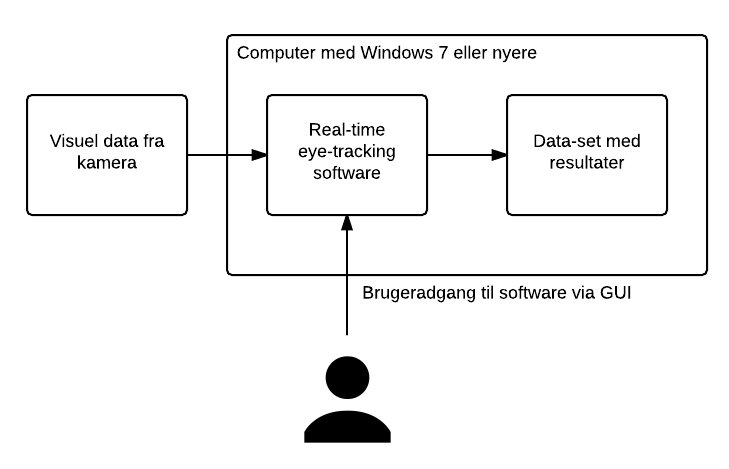
\includegraphics[width=0.7\linewidth]{../Systemdiagram.png}
\caption[Systemdiagram]{Systemdiagram for Real-time eye-tracking}
\label{fig:Systemdiagram}
\end{figure}
Der ønskes udviklet et system som kan indsamle videodata fra et kamera og derefter anvende dataen til
at bestemme hvor en forsøgsperson kigger hen på en specifik skærm. Systemet skal derudover videregive
denne information til brugeren via koordinater samt en graf der repræsenterer den skærm forsøgspersonen
ser på.
\\
\indent
Før dataopsamling skal en indledende kalibrering af systemet gennemføres. Dette gøres ved at et gitter med
specifikke punkter indlæses på forsøgspersonsskærmen. Derefter bedes forsøgspersonen fiksere på specifikke punkter
på skærmen, og sammenhængen imellem de målte punkter og de kendte punkter kan anvendes til at finde en
homografisk mapning. Efter denne kalibrering kan systemet anvendes.
\\
\indent
Systemet udvikles med henblik på en standard anvendelsesmåde, med mulighed for brugerdefinerede anvendelsesmåder. 
Standardanvendelsen omhandler at vælge en sti og et filnavn, hvorefter dataopsamling umiddelbart begynder.
Under dataopsamlingen vil gazevectoren løbende blive præsenteret for brugeren på brugerskærmen. Når brugeren er 
færdig kan opsamlingen stoppes, og dataopsamlingen gemmes i den tidligere valgte fil. Bemærk at den algoritme
der anvendes til behandling af data her er forudbestemt.
\\
(Hvis brugeren ønsker at bruge en anden algoritme kan denne indlæses. Den kan også indskrives direkte i
GUI'en, og derefter gemmes. Formålet med dette er at kunne indrette systemet efter specifikke behov, og
hurtigt indhente de opsætninger til fremtidig brug. Eventuelt kan andre variabler indtastes ved systemstart) 
\\
\indent
I de følgende afsnit fremgår det hvorledes det udviklede system indgår i det samlede system.


\subsection{Aktører}
\begin{figure}[h]
\centering
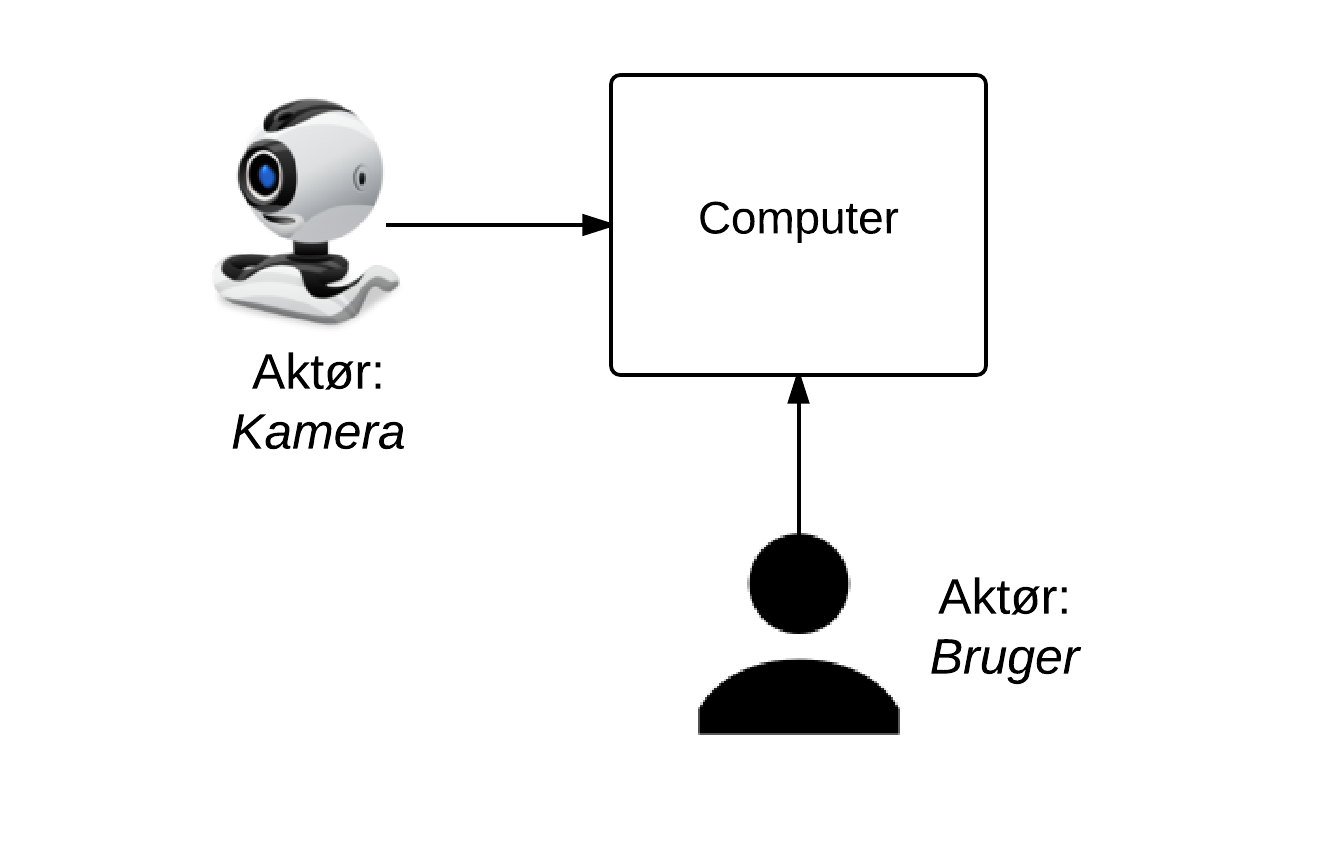
\includegraphics[width=0.7\linewidth]{../Actors}
\caption{Systemets aktører}
\label{fig:Actors}
\end{figure}

En række af de kommende funktionelle krav vil blive opstillet som use-cases. Følgende er beskrivelser for de enkelte aktører: \\
\\
\begin{tabular}{| l | p{10cm} |}
	\hline 
	\textbf{Navn} & \textit{Bruger} \\ \hline
	\textbf{Beskrivelse} & Brugeren er personen der tilgår systemet via et grafisk user interface.\\ \hline
\end{tabular}
\newline
\vspace*{0.7 cm}
\newline
\begin{tabular}{| l | p{10cm} |}
	\hline 
	\textbf{Navn} & \textit{Kamera} \\ \hline
	\textbf{Beskrivelse} & Systemet vil snakke sammen med et kamera, hvis formål er at levere visuelt data.\\ \hline
\end{tabular}

\subsection{Systemets begrænsninger}
\begin{enumerate}
	\item Systemet kan ikke forventes at køre realtime (100 fps) udenfor standard anvendelse.
\item 
Systemet er ikke garanteret at fungere korrekt når testpersonen har briller på.
\item 
Systemet kan ikke anvendes uden indledende kalibrering.
\item 
Systemet kan ikke håndtere hovedbevægelser uden for $\pm10$ cm i forhold til kalibreringspositionen.
\end{enumerate}
>>>>>>> origin/master
\end{document}